\chapter{Rozbor řešené problematiky}

\section{Webové portály}
Webový portál je druh webové stránky, která shromažďuje informace z vícero různých zdrojů a uživateli ty nejrelevantnější informace prezentuje uživateli shromážděné na jednom místě %[https://www.liferay.com/resources/l/web-portal 20. 4.]. 
Zpravidla je umožněno na portálu v těchto informací vyhledávat. Velmi časté je také zakomponování autentizace uživatele a podle jeho role jsou mu zpřístupněny různé části daného portálu. %[https://kb.iu.edu/d/ajbd]
\blindtext[2]

\subsection{Cordis}
%[https://cordis.europa.eu/about/]
The Community Research and Development Information Service je portál provozovaný Evropskou Unií (dále jen EU) sloužící jako hlavní zdroj výsledků projektů, sponzorovaných v rámci programů EU pro výzkum a inovaci. Na jednom místě veřejně poskytuje informace jak o těchto projektech, tak i o jejích účastnících, o hlášeních, vědeckých zprávách a publikacích.
\blindtext

\subsection{Funding and Tenders}
\blindtext

\section{Python}
\blindtext[2]

\section{Flask}
%[http://flask.pocoo.org/docs/1.0/foreword/ 21.4.]
Flask je open source webový micro-framework napsaný v programovacím jazyce Python. Klíčový znak micro-frameworků je co nejmenší nebo i nulová závislost na externích knihovnách %[https://pymbook.readthedocs.io/en/latest/flask.html 23.4.]
Flask si si klade za cíl udržet co nejjednodušší jádro, ale zároveň se soustředí na možnost tento základ jednoduše rozšířit.
Smyslem Flasku je být základním kamenem pro jakoukoliv webovou aplikaci. Z tohoto důvodu na rozdíl od ostatních frameworků neobsahuje žádnou abstrakci databázové vrstvy nebo knihovnu pro formuláře. Tohoto lze docílit použitím některého z rozšíření %[http://flask.pocoo.org/docs/1.0/design/ 23. 4.] 

Ve svém základu využívá šablonovací jazyk Jinja2 zjednodušující udržení konzistentní struktury stránek. Poskytuje například dědičnost šablon nebo znovupoužitelné bloky a dokáže se vypořádat s bezpečnostními útoky typu XSS (Cross Site Scripting). %[http://jinja.pocoo.org/docs/2.10/]
Druhou knihovnou, kterou Flask využívá je Werkzeug - jedna z nejpokročilejších knihoven pro rozhraní brány webového serveru (anglicky WSGI neboli Web Server Gateway Interface), které umožňuje webovou aplikaci provozovat nezávisle na technologii použité na serveru. %[https://www.python.org/dev/peps/pep-0333/#rationale-and-goals]

Tento framework využívá například sociální síť Pinterest %[https://www.quora.com/What-challenges-has-Pinterest-encountered-with-Flask/answer/Steve-Cohen?share=1&srid=hXZd 23.4.]
nebo síťová dopravní společnost Lyft %[https://www.youtube.com/watch?v=aetoXWRt24k]
(podobná službě Uber)

\section{Vue}
V dnešní době jsou webové prohlížeče stále schopnější a výkonnější. Díky tomu se stává trendem přenášet stále větší části webové aplikace ze serveru na stranu klienta. Toho je docíleno pomocí programovacího jazyku JavaScript. V současné době se nejvíce využívá knihovna jQuery, %[Todo: najít zdroj]
ale začali se objevovat pokročilejší frameworky jako například React, Angular a v neposlední řadě Vue.

Vue je progresivní framework - přizpůsobuje se složitosti projektu. Podobně jako dříve zmiňovaný Flask se nejedná o rozsáhlý framework, jehož části by jste vypínali, ale jedná se o základní framework, který můžete dále rozšiřovat %[http://slides.com/evanyou/progressive-javascript#/18 23.4.]
Díky tomuto přístupu učební křivka není tak strmá, jako u konkurenčních frameworků. Jediné, co člověku pro začátek práce s Vue stačí je být obeznámen s HTML a s čistým JavaScriptem.  %[https://vuejs.org/v2/guide/comparison.html#Learning-Curve  24.4.]

Jedna z předností toto frameworku je jednoduchost obousměrné vazby dat. Tato vazba znamená, že hodnota proměnné v jazyce JavaScript je synchronizována s hodnotou v objektovém modelu dokumentu (DOM) a to stejné platí i v opačném směru. %[https://medium.com/js-dojo/exploring-vue-js-reactive-two-way-data-binding-da533d0c4554 24.4.]
V praxi může být tato funkce využita například v internetovém obchodě, kdy uživatel klikne na tlačítko \uv{Přidat do košíku}, které pouze rozšíří pole košíku o další produkt. Bez jakéhokoliv dalšího úsilí komponenty, závislé na této proměnné zaznamenají změnu a automaticky provedou odpovídající akce - košík přepočítá celkový počet vybraného zboží, celkovou cenu nákupu, zlevní se cena daného produktu, při koupi dalších kusů apod. 

\subsection{Vue Router}
Mezi oficiálně podporované knihovny patří například Vue Router, umožňující tvorbu jednostránkové aplikace, kdy se načte pouze jedná jediná stránka a pomocí JavaScriptu a asynchroniích požadavků se mění části obsahu webu. Server v takovém případě slouží pouze jako úložiště dat a veškerou prezentaci se stará strana klienta. %[https://msdn.microsoft.com/en-us/magazine/dn463786.aspx 24.4.]

\subsection{Vuex}
%[https://vuex.vuejs.org/ 24.4.]
Dalším oficiálním rozšířením je Vuex, knihovna pro správu stavu. Pokud se v aplikaci používá více komponent, které využívají stejnou proměnnou, brzy se zdrojový kód stává neudržitelným. 
V tuto chvíli je vhodné využit knihovnu Vuex. Jejím účelem je udržovat centrální stav proměnných, které jsou sdíleny napříč různými komponentami v aplikaci. Tohoto je docíleno díky dodržování návrhového vzoru jménem Flux. Mezi základní pilíře návrhového vzoru Flux patří několik následujících pravidel, kterých se Vuex drží. 
%TODO: Reference na MVC


%[https://medium.com/js-dojo/vuex-for-the-clueless-the-missing-primer-on-vues-application-data-store-33fa51ffc3af 25.4.]
\subsubsection*{Jediný zdroj pravdy}
Data, která jsou sdílena více komponentami jsou uložena na jednom místě - sklad (anglicky \emph{store}) a jsou oddělena od komponent, které jé využívají. Komponenty mohou stále mít svá lokální data, ale nesmějí mít svou kopií sdílených dat, ty se vždy musí číst ze skladu.

\subsubsection*{Data pouze ke čtení}
Komponenty nesmějí přímo upravovat data ve skladu. V případě potřeby změny těchto dat sklad pouze informují a ten se sám o postará o provedení změny pomocí tzv. mutací (Reprezentovány uzlem \emph{Mutations} v grafu \ref{vuex-dataflow}). Díky tomu se minimalizuje šance nepředpokládaných změn těchto dat a funkce, starající se o tyto změny jsou jednodušeji dohledatelné.

%TODO: AddToCart mutation example?

\subsubsection*{Změny dat jsou synchronní}
Asynchronní provádění operací mnohdy přináší spoustu výhod, v tomto případě je ale vyžadováno mutace provádět synchronně kvůli odstranění závislosti na pořadí a načasování různých událostí.


\begin{figure}[H]
	\centering
	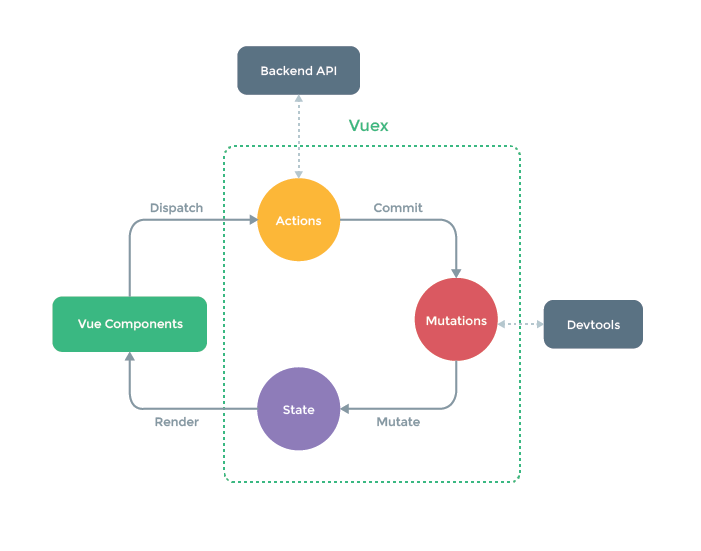
\includegraphics[width=\textwidth]{images/vuex.png}
	\caption{Diagram znázorňující životní cyklus dat v knihovně Vuex}
	%TODO: Popsat v obrázku nebo v textu?
	%[https://vuex.vuejs.org/ 24.4.]
	\label{vuex-dataflow}
\end{figure}

\blindtext

\section{Elasticsearch}
Elasticsearch je volně šiřitelný vyhledávač umožňující rychlé vyhledávání ve velkém množství dat. 

Oproti relačním databázím nenabízí propojovací dotazy, a proto je nutné ukládaná data denormalizovat. Díky tomu jsou ale data a jejich metadata v těsné blízkosti a tím je docíleno rychlé fulltextové vyhledávání. %[https://qbox.io/blog/what-is-elasticsearch 20.4.]

\subsection{Dotazy}
Pro komunikaci s touto databází se využívá Query DSL - dotazy aplikačního rozhraní REST ve formátu JSON.

Obsah dotazu může vypadat například následovně:
\begin{verbatim}
{
    "query": {
        "match": {
            "address": "mill lane"
        }
    }
}
\end{verbatim}

Na tento dotaz můžeme od serveru dostat tuto odpověď
\begin{verbatim}
\blindtext
\end{verbatim} 

\subsubsection*{Kontext}
Dotazy v Elasticsearch se rozlišují na dva základní typy - kontext dotazu (query) a kontext filtru.
První z nich se dá lidsky přeložit do otázky \uv{Jak moc dokument splňuje dotaz?}. V tomto případě se u každého výsledku počítá skóre relevance, podle kterého jsou ve výsledné odpovědi dokumenty sestupně řazeny.


\subsection{Základní struktura}
Základní struktura databáze Elasticsearch se na první pohled od tradičních relačních databázi velmi neliší, ke spoustě pojmů se dá najít ekvivalent.

\subsubsection*{Uzel a shluk}
Pod pojmem uzel (anglicky node) se skrývá server, ve kterém jsou uložena data. Uzel v rámci databáze může být jeden nebo jich může být i více a každý bude obsahovat pouze určitou část dat. Tyto uzly jsou seskupeny do shluku (anglicky cluster).


\subsubsection*{Dokument}
Dokument je základní jednotka dat, které může být zaindexována. Obsah dokumentu je zapsán ve formátu JSON. V relační databázi lze dokument přirovnat k řádku tabulky.

\subsubsection*{Index}
Skupina dokumentů s podobnou strukturou se nazývá index. Ekvivalentem v relačních databázich by v tomto případě byla tabulka.

\subsubsection*{Střepy}
Elasticsearch nabízí možnost index rozdělit na střepy (anglicky shards), které mohou být uloženy v různých uzlech. Tuto možnost je vhodné využít především při práci s indexy s velkým obsahem dat. Díky rozdělení docílíme distribuování zátěže a lze využít paralelní zpracování, tudíž bude zpracování dotazu odbaveno výrazně rychleji. 
Přístup k takto rozděleným indexům se nijak nemění a pro uživatele je tento proces naprosto transparentní.

\subsubsection*{Repliky}
Obdobně lze využít i repliky. Zde se ovšem data indexu nerozdělují, ale naopak duplikují. Díky uložení těchto replik mezi více uzly může systém být robustnější a dokáže fungovat i v případě selhání části shluku. I v tomto případě je umožněno vyhledávat paralelně. 

\subsection{Fasetové vyhledávání}
S velkým množstvím dat přichází potřeba obsah podle určitých kriterií zúžit. K tomotu účelu slouží filtry a fasetové vyhledávání (někdy také označována jako fastová navigace - anglicky faceted search nebo faceted navigation). Využití faset je ale pokročilejší než použít filtry, protože fasetová navigace umožňuje využít hned několik filtrů najednou. %[https://www.nngroup.com/articles/filters-vs-facets/ 21.4.]

V Elasticsearch je možné tuto navigaci vytvořit pomocí tzv. kyblíkových agreagací (angl. bucket aggregations).
Jednoduše řečeno, se pro dokumenty vytvoří kyblíky, kde každý z kyblíku odpovídá určitému kriteriu. Pokud dokument toto kriterium splňuje, je do kyblíku vložen.
%[https://www.elastic.co/guide/en/elasticsearch/reference/current/search-aggregations-bucket.html 21.4.]

\subsection{Plnotextové vyhledávání}
\blindtext[2]

\subsection{Podobnostní hledání}
\blindtext[2]


\section{Vývoj webu}
\subsection{MVC architektura}
%[https://pdfs.semanticscholar.org/9077/6c1fd8c2c4dbd13b85f22e7c8c8f83331758.pdf 27.4.]
Většinu aplikací lze obecně rozdělit na tři hlavní celky - data, rozhraní a logiku. V anglickém jazyce se tyto celky dají nazvat pomocí slov \emph{model}, \emph{view} a \emph{controller} (zkratka MVC). Historie této architektury sahá až do sedmdesátých let, nicméně je tato architektura v dnešním světe stále naprostým standardem vývoje.

\begin{figure}[H]
	\centering
	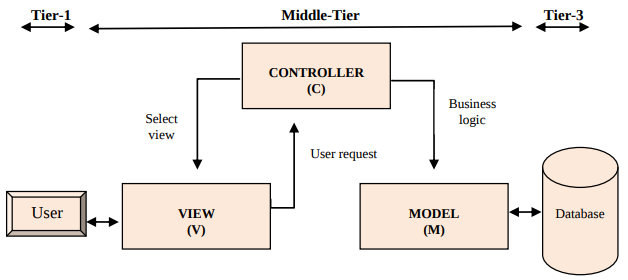
\includegraphics[width=\textwidth]{images/mvc.png}
	\caption{Diagram toku akcí při využití MVC architektury}
	\label{mvc}
\end{figure}

\begin{itemize}
\item Pojmem pohled (\emph{view}) se označuje uživatelské rozhraní (například stránka zobrazená v prohlížeči), tato vrstva prezentuje data a je to také jediná vrstva, s kterou uživatel přímo komunikuje. Akce provedené v pohledu se předají kontroleru ke zpracovaní.
\item Kontroler ((\emph{controller}) se chová jako prostředník mezi daty a rozhraním, zpracovává požadavky uživatele a provede s modelem potřebné akce. Ve většině případu po provedené akci kontroler znovu obnoví pohled.
\item Model je obvykle objekt obsahující patřičná data z databáze. Zprostředkovává jak jejich získání, tak i ukládání. Mimo to může být objekt obohacen i o funkce, zpracovávající tyto data (například může převádět Unixový čas do formátu lépe čitelného pro člověka). 
\end{itemize}


Oddělením těchto celků je zajištěna lepší organizovanost zdrojových kódů a tím je usnadněn rychlejší vývoj. Jednotlivé celky jsou také lehčeji znovupoužitelné a práce programátorů na nich může probíhat souběžně. Rozdělením je také možné pro jeden pohled mít pohledů hned několik. Další pohledy mohou přibývat nebo naopak ty stávající mohou být smazány a na databázi aplikace to nebude mít žádný vliv.

\subsection{Responsivita}
\blindtext[2]